\section{Versuchsaufbau und Durchführung}
\label{sec:Durchführung}

Der in diesem Versuch verwendete Aufbau ist in Abbildung \ref{fig:Aufbau} dargestellt. Das
zu untersuchende Licht stammt von einer Cd-Lampe, welche dem Magnetfeld eines Elektromagneten
ausgesetzt ist. Senkrecht zum Magnetfeld wird das Licht mit Linsen, Spalten und einem
Gradschichtprisma nach Wellenlängen aufgespalten. Mit einem Spalt kann dann die gewünschte Linie
ausgewählt werden. Die gewünschte Polarisation wird mit einem Polarisationsfilter herrausgefiltert.
Das Licht wird nun auf eine Lummer-Gerschke-Platte geleitet, welche ein Interferenzmuster erzeugt.
Für monochromatisches Licht erzeugt die Lummer-Gerschke-Platte einen Gangunterschied von $\lambda$.
Da sich bei eingeschaltetem Magnetfeld die Wellenlänge um $\delta \lambda$ ändert, verschieben sich
demzufolge auch die Interferenzstreifen um $\delta s$.
\begin{figure}
  \centering
  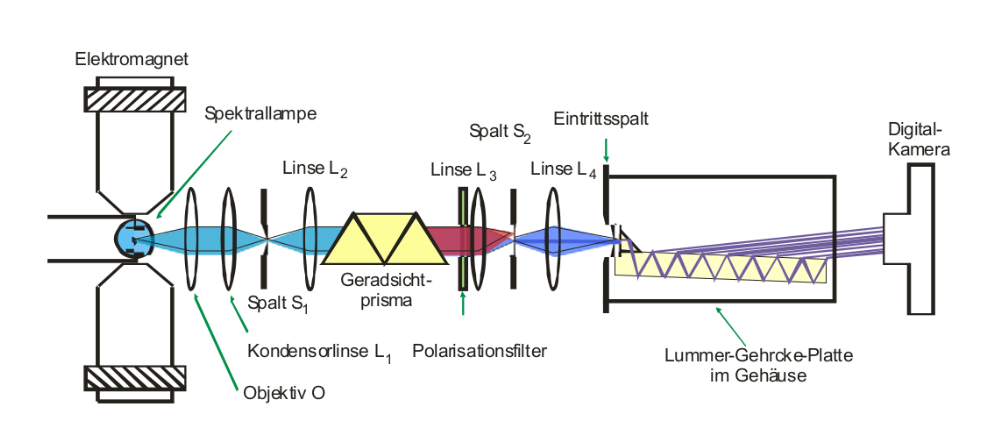
\includegraphics[width=11cm]{Aufbau.png}
  \caption{Verwendeter Versuchsaufbau \cite{skript}.}
  \label{fig:Aufbau}
\end{figure}

Damit sich zwei Wellenlängen nicht überlagern, darf die Wellenlänge
das Dispersionsgebiet
\begin{equation}
  \Delta\lambda_D=\frac{\lambda^2}{2\cdot d}\sqrt{\frac{1}{n^2-1}}
  \label{eqn:dispersion}
\end{equation}
nicht überschreiten. Dabei bezeichnet $d$ die Dicke der Platte und
$n$ die Ordnung des Maximums.
Das Auflösungsvermögen A der Lummer-Gerschke-Platte kann über die Formel
\begin{equation}
  A=\frac{L}{\lambda}(n^2-1)
  \label{eqn:Auflösung}
\end{equation}
bestimmt werden. Dabei ist $L$ die Länge der Platte und $n$ der Brechungsindex.

Um die aufgespaltenen Spektrallinien messen zu können, wird zunächst das Magnetfeld des
Elektromagneten geeicht. Dazu wird das Magnetfeld in Abhängigkeit des angelegten Stroms
im Intervall $0<I<\SI{19}{\A}$ mit einer Hall-Sonde vermessen. Anschließend wird der
Aufbau justiert, sodass die Wellenlängen, welche über einen Spalt ausgewählt werden können, auf
die Lummer-Gerschke-Platte treffen. Mithilfe des Polarisationsfilters kann die
gewünschte Polarisation ausgewählt werden.
Die Messung wird für die rote und blaue Linie des Cd-Spektrums duruchgeführt. Dazu wird
eine Digitalkamera hinter der Lummer-Gerschke-Platte aufgestellt, mit der das Interferenzbild
fotografiert werden kann. Es werden Bilder bei verschiedenen Polarisationen und
Magnetfeldstärken aufgenommen, um die Wellenlängenverschiebung zu bestimmen.
